\documentclass[letter,11pt]{article}

\usepackage[spanish,es-nodecimaldot]{babel}
\usepackage[utf8]{inputenc}

\usepackage{lmodern}
\usepackage[T1]{fontenc}
\usepackage{textcomp}

\usepackage{framed}
\usepackage[svgnames]{xcolor}

\usepackage{graphicx}
\usepackage{pstricks}

\usepackage{anysize}
\marginsize{3cm}{2cm}{2cm}{3cm}

\usepackage{siunitx}
\usepackage{amsmath}
\usepackage{array}

\usepackage{fancyhdr}
\usepackage{lastpage}
\pagestyle{fancy}
\fancyhf{}
\fancyhead[LE,RO]{Física Básica III}
\fancyfoot[CO,CE]{\thepage\ de \pageref{LastPage}}

\special{papersize=215.9mm,279.4mm}

\usepackage[
    pdfauthor={Carlos Eduardo Caballero Burgoa},%
    pdftitle={Física Básica III},%
    pdfsubject={1er Parcial},%
    colorlinks,%
    citecolor=black,%
    filecolor=black,%
    linkcolor=black,%
    urlcolor=black,
    breaklinks]{hyperref}
\usepackage{breakurl}

\newcommand{\blankpage}{
\newpage
\thispagestyle{empty}
\mbox{}
\newpage
}

\renewcommand{\arraystretch}{1.2}

\begin{document}

\begin{center}
    {\Large \bf{Practica primer parcial}}
\end{center}

\noindent\fbox{%
    \parbox{\textwidth}{%
        Estudiante: CABALLERO BURGOA, Carlos Eduardo \\
        Carrera: Ingeniería Electromecánica \\
        Correo: cijkb.j@gmail.com
    }%
}

\vspace{0.5cm}

\begin{enumerate}
\item Calcula la densidad superficial de carga en la superficie externa ($r=b$),
de un cascaron conductor que tiene una carga total de $10[\mu C]$, si en el
interior del cascaron se encuentra una esfera aislante de radio $a$ y con
densidad de carga volumétrica uniforme de $20[\mu C/m^3]$. Considera $a=0.1[m]$
y $b=0.3[m]$.

\begin{itemize}
    \item \textcolor{purple}{$\sigma = 8.92 [\mu C/m^2]$}.
    \item $\sigma = 0.92 [\mu C/m^2]$.
    \item $\sigma = 4.02 [\mu C/m^2]$.
    \item Ninguno.
\end{itemize}

\textbf{Solución:}

%\begin{figure}[!h]
%\centering
%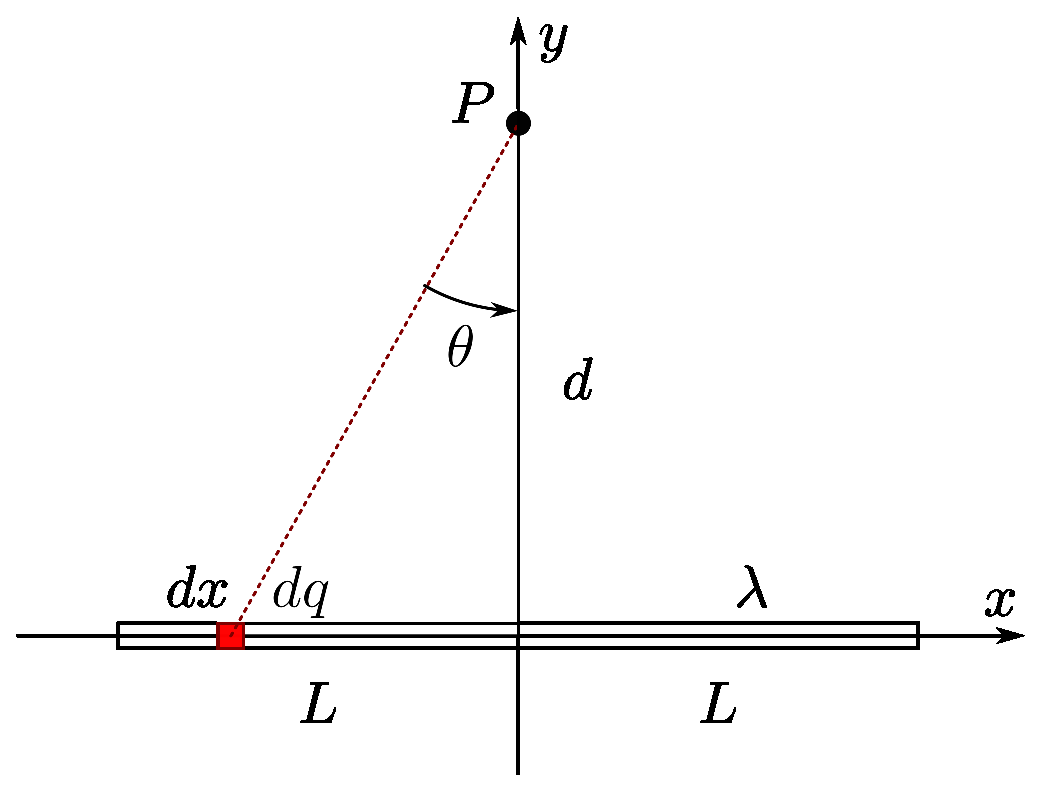
\includegraphics[scale=0.39]{resources/a1.eps}
%\end{figure}

\item Una barra delgada de longitud $L$ lleva una densidad de carga lineal
uniforme $\lambda$ se ubica sobre el eje $X$, desde $x=L$ hasta $x=2L$, si esta
dentro de un campo eléctrico dado por: $\vec{E}=\dfrac{1}{x^2} \hat{u}_y$,
calcula la fuerza eléctrica que actúa sobre la barra.

\textbf{Solución:}

\item Se colocan dos cargas como se muestra en la figura. La magnitud de $q_1$
es de $3[\mu C]$ pero se desconoce el signo y el valor de la carga $q_2$. La
dirección del campo eléctrico neto en el punto $P$ esta enteramente en la
dirección $Y$ negativa. Calcula la magnitud del campo eléctrico.

\begin{itemize}
    \item $E=1.17[N/C]$.
    \item $E=\num{0.17e7}[N/C]$.
    \item $E=\num{1.17e7}[N/C]$.
    \item Ninguno.
\end{itemize}

\textbf{Solución:}

\item Se tiene una distribución de carga compuesta de: un alambre infinito
vertical con $\num{e-6}[C/m]$ de densidad lineal de carga uniformemente
distribuida y una esfera de $1[m]$ de radio con densidad volumétrica de carga
dada por: $\rho=A\,r$, donde $A=\num{e-6}[C/m^4]$, cuyo centro se encuentra a
$3[m]$ del alambre infinito, como se muestra en la figura. Calcula el modulo del
campo eléctrico total a $1[m]$ del alambre infinito sobre la linea que une el
alambre y el centro de la esfera.

\textbf{Solución:}

\item Si una carga $-2q$ se encuentra en el origen de coordenadas, otra carga
$q$ se encuentra en $(a,0)$ y una tercera carga $q$ se encuentra en $(-a,0)$,
calcula el campo eléctrico en la posición $(0,y)$ considerando que $y>>a$.

\begin{itemize}
    \item $\vec{E}=-\dfrac{3qa^2}{4\pi\epsilon_0 y^4}\hat{u}_y$.
    \item $\vec{E}=\dfrac{qa^2}{4\pi\epsilon_0 y^4}\hat{u}_y$.
    \item $\vec{E}=-\dfrac{3qa^2}{4\epsilon_0 y^4}\hat{u}_y$.
    \item Ninguno.
\end{itemize}

\textbf{Solución:}

\item La carga $Q$ esta distribuida uniformemente a lo largo del eje positivo
$Y$ entre $y=0$ y $y=a$, otra carga puntual $-q$ se encuentra en el eje positivo
$X$, a una distancia $x$ del origen. Calcula la magnitud de la fuerza que la
distribución de carga $Q$ ejerce sobre $-q$.

\begin{itemize}
    \item $\vec{F}=\dfrac{qQ}{4\pi\epsilon_0}\Biggr[-\dfrac{\hat{u}_x}{x\sqrt{x^2+a^2}}+\Biggr(\dfrac{1}{x}-\dfrac{1}{\sqrt{x^2+a^2}}\Biggr)\hat{u}_y\Biggr]$
    \item $\vec{F}=\dfrac{qQ}{4\pi\epsilon_0}\Biggr[-\dfrac{\hat{u}_x}{x\sqrt{x^2+a^2}}+\dfrac{1}{a}\Biggr(-\dfrac{1}{\sqrt{x^2+a^2}}\Biggr)\hat{u}_y\Biggr]$
    \item $\vec{F}=\dfrac{qQ}{4\pi\epsilon_0}\Biggr[-\dfrac{\hat{u}_x}{x\sqrt{x^2+a^2}}+\dfrac{1}{a}\Biggr(\dfrac{1}{x}-\dfrac{1}{\sqrt{x^2+a^2}}\Biggr)\hat{u}_y\Biggr]$
    \item Ninguno.
\end{itemize}

\textbf{Solución:}

\end{enumerate}
\end{document}

